\subsection{Pengenalan IO: LED, push button dan seven segment}

\subsubsection{LED}

LED merupakan output yang paling sederhana pada board FPGA yang akan
kita gunakan. Salah satu tujuan utama dari eksperimen ini adalah
untuk mengetahui keadaan LED apabila diberikan nilai logika 0 dan 1.
Hal ini lebih mudah dilakukan dengan menggunakan Verilog.
Kita juga akan mempelajari sintaks Verilog untuk


Buat file baru, misalnya dengan nama \textbf{led\_light.v}.
\textit{Hindari nama file dengan menggunakan spasi}.
Kemudian ketik kode Verilog berikut pada file tersebut.
Kode Verilog ini memberikan nilai logika ke tiap
LED (hardwired, tanpa ada input).

{\setstretch{1.0}
\begin{verilogcode}
module led_light(led);
  output [3:0] led;
  assign led = 4'b0000; // coba ubah-ubah nilai ini untuk tiap LED
endmodule
\end{verilogcode}
}

Compile file ini dengan cara klik icon \textbf{Compile} atau dengan menu
\textbf{Processing $\rightarrow$ Start Compilation} atau menggunakan shortcut
\textbf{Ctrl + L}.

Jika tidak ada kesalahan pada saat proses kompilasi,
maka langkah selanjutnya adalah melakukan
PIN assignment, yang dapat dilakukan dengan memilih menu
\textbf{Assignment $\rightarrow$ Pin Planner} atau menggunakan shortcut
\textbf{Ctrl + N}.

Berikut ini adalah data PIN yang diberikan.

\begin{table}[H]
\caption{Data PIN untuk LED}\label{tab:pin}
\centering
\begin{tabular}{|c|c|}
\hline 
\multicolumn{2}{|c|}{LED} \\
\hline 
LED1 & PIN\_87 \\
\hline 
LED2 & PIN\_86 \\
\hline 
LED3 & PIN\_85 \\
\hline 
LED4 & PIN\_84 \\
\hline 
\end{tabular}
\par
\end{table}

Atur PIN assigment sesuai dengan keperluan.
Jendela PIN assignment ini dapat dibiarkan terbuka.

\begin{figure}[H]
\centering
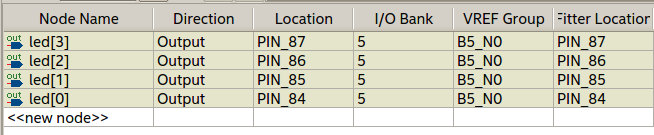
\includegraphics[scale=0.5]{images/PinPlanner_4LED.png}
\par
\caption{Contoh PIN Assignment untuk 4 LED, mohon disesuaikan dengan
kode Verilog dan board yang digunakan}
\end{figure}

\textit{Compile lagi file tersebut setelah PIN assignment dilakukan}.

Jika tidak ada pesan error, langkah selanjutnya adalah mendownload program
ini ke FPGA. Proses ini dapat dilakukan dengan cara memilih menu
\textbf{Tools $\rightarrow$ Programmer}.
Klik button \textbf{Add File} untuk menambahkan file {\tt led\_light.sof}.
File ini biasanya ada di dalam subdirektori {\tt output} dari direktori
proyek.
Pastikan juga hardware telah terdeteksi. Jika belum terdeteksi, tambahkan melalui
dengan mengklik button \textbf{Hardware Setup}.

\begin{figure}[H]
\centering
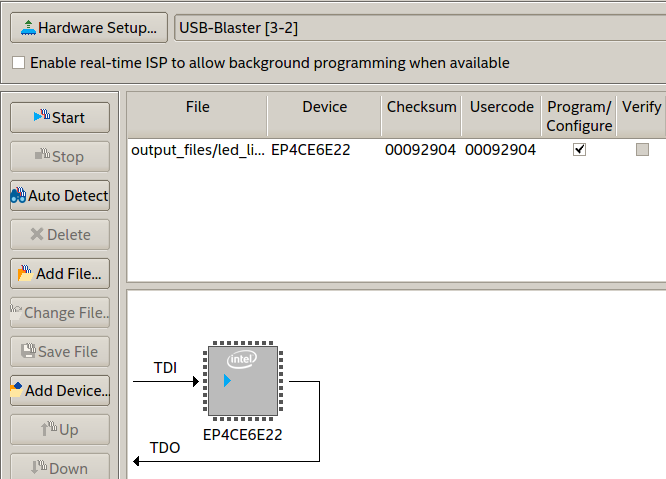
\includegraphics[scale=0.4]{images/Programmer_4LED.png}
\par
\caption{Tampilan tool \textbf{Programmer}}
\end{figure}

Misalkan pada board FPGA yang digunakan urutan LED dari kiri ke kanan adalah LED1,
LED2, LED3, dan LED4.

Misalkan memberikan assignment sebagai berikut.
\begin{itemize}
\item LED1 diwakili dengan {\tt led[0]}
\item LED2 diwakili dengan {\tt led[1]}
\item LED3 diwakili dengan {\tt led[2]}
\item LED4 diwakili dengan {\tt led[3]}
\end{itemize}


Misalkan juga kita memberikan nilai logika pada {\tt led} dengan
kode Verilog berikut.
\begin{verilogcode}
  led = 4'b1010;
\end{verilogcode}
Maka nilai 0 (nilai bit paling kanan atau LSB) diberikan pada {\tt led[0]}
atau LED1. Nilai pada bit kedua dari kanan diberikan untuk {\tt led[1]}, bit ketiga
untuk {\tt led[2]}, dan bit keempat (paling kiri atau MSB) untuk {\tt led[3]}.

Bagian {\tt output [3:0] led} pada kode di atas dapat diganti
dengan {\tt output [1:4] led} untuk memudahkan assignment nilai logika
sesuai dengan urutan LED di board yang digunakan. Sehingga kita dapat
melakukan assigment sebagai berikut.
\begin{itemize}
\item LED1 diwakili dengan {\tt led[1]}
\item LED2 diwakili dengan {\tt led[2]}
\item LED3 diwakili dengan {\tt led[3]}
\item LED4 diwakili dengan {\tt led[4]}
\end{itemize}


Cobalah bereksprimen dengan cara mengganti-ganti nilai logika
dari {\tt led}, kemudian isilah tabel berikut.

\begin{table}[H]
\centering
\begin{tabular}{|c|c|}
\hline
Nilai logika & Keadaan LED (on/off) \\
\hline
0 & \\
1 & \\
\hline
\end{tabular}
\par
\end{table}

Untuk penggunaan berikutnya, isikan juga PIN untuk LED, sesuai dengan
letaknya di board FPGA. Dari kiri ke kanan:

\begin{table}[H]
{\centering
\begin{tabular}{|c|c|c|c|}
\hline
PIN: \hspace{2cm} & PIN: \hspace{2cm} & PIN: \hspace{2cm} & PIN: \hspace{2cm} \\
\hline
\end{tabular}
\par}
\end{table}

\subsubsection{Push buttons}

Setelah mengetahui keadaan LED jika diberikan nilai logika 0 dan 1, kita
dapat mengetahui keadaan logika push button apabila dilepas dan ditekan.

Buat file Verilog baru dengan mendefiniskan satu modul
dengan input dari push button dan output ke LED.

\begin{verilogcode}
module test_buttons( buttons, led );
  input  [3:0] buttons;
  output [3:0] led;

  assign led = buttons;
endmodule
\end{verilogcode}

Bisa juga menggunakan potongan kode berikut.
\begin{verilogcode}
  assign led[0] = buttons[0];
  assign led[1] = buttons[1];
  assign led[2] = buttons[2];
  assign led[3] = buttons[3];
\end{verilogcode}

Cobalah bereksperimen dengan kode Verilog yang ada dan juga menggukan operator Verilog
seperti 

\begin{table}[H]
\centering
\begin{tabular}{|c|c|}
\hline
Nilai logika & Keadaan PB \\
\hline
0 & \\
1 & \\
\hline
\end{tabular}
\par
\end{table}

Untuk penggunaan berikutnya, isikan juga PIN untuk push button,
sesuai dengan letaknya di board FPGA. Dari kiri ke kanan:

\begin{table}[H]
{\centering
\begin{tabular}{|c|c|c|c|}
\hline
PIN: \hspace{2cm} & PIN: \hspace{2cm} & PIN: \hspace{2cm} & PIN: \hspace{2cm} \\
\hline
\end{tabular}
\par}
\end{table}


\subsubsection{Seven segments}

Lihat juga Modul 1.

Berikut ini adalah tabel nomor PIN terkait dengan seven-segment display
yang diberikan oleh distributor FPGA.

\begin{table}[H]
\caption{Port Seven-segment LED}\label{tab:pin_sseg}
\centering
\begin{tabular}{|c|c|}
\hline 
\multicolumn{2}{|c|}{Seven-segment LED} \\
\hline 
DIG1 & PIN\_133 \\
\hline 
DIG2 & PIN\_135 \\
\hline 
DIG3 & PIN\_136 \\
\hline 
DIG4 & PIN\_137 \\
\hline 
SEG0 & PIN\_128 \\
\hline 
SEG1 & PIN\_121 \\
\hline 
SEG2 & PIN\_125 \\
\hline
SEG3 & PIN\_129 \\
\hline
SEG4 & PIN\_132 \\
\hline
SEG5 & PIN\_126 \\
\hline
SEG6 & PIN\_124 \\
\hline
SEG7 & PIN\_127 \\
\hline 
\end{tabular}
\par
\end{table}

Seperti pada percobaan sebelumnya, buat file Verilog dengan konten sebagai berikut.
Lengkapi kode tersebut dan modifikasi bagian yang Anda perlukan.

\begin{verilogcode}
module tes_sseg(
  output [7:0] sseg,
  output [3:0] en_dig
);

  assign sseg[7] = 0;
  // lengkapi jika diperlukan
  assign sseg[0] = 1;
  
  assign en_dig[3] = 1;
endmodule
\end{verilogcode}

\begin{figure}[H]
\centering
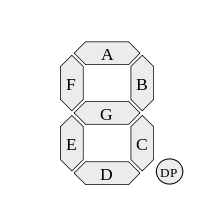
\includegraphics[scale=0.5]{images/sseg.png}
\par
\caption{Seven segment}\label{fig:sseg}
\end{figure}

Untuk referensi lebih lanjut isilah tabel berikut. dengan memperhatikan Gambar
\ref{fig:sseg}.

\begin{table}[H]
\centering
\begin{tabular}{|c|c|}
\hline
Segmen & PIN \\
\hline
A & \\
\hline
B & \\
\hline
C & \\
\hline
D & \\
\hline
E & \\
\hline
F & \\
\hline
G & \\
\hline
DP & \\
\hline
\end{tabular}
\end{table}
